\section{Auswertung}
\label{sec:Auswertung}

\subsection{Detektorscan}
 Um aus dem Detektorscan die Halbwertsbreite 
 und die maximale Intensität bestimmen zu können wird eine Gaußfunktion
 \begin{equation}
     I(\alpha) = \frac{1}{\sqrt{2\pi \sigma^2}}\exp\left(-\frac{(\alpha - \mu)^2}{2\sigma^2}\right)
 \end{equation} 
an die Messwerte genährt.
Die gemessene Werte mit der dazugehörigen Gaußdistribution sind in Abbildung \ref{fig:gauß} dargestellt.
\begin{figure}[ht]
    \centering
    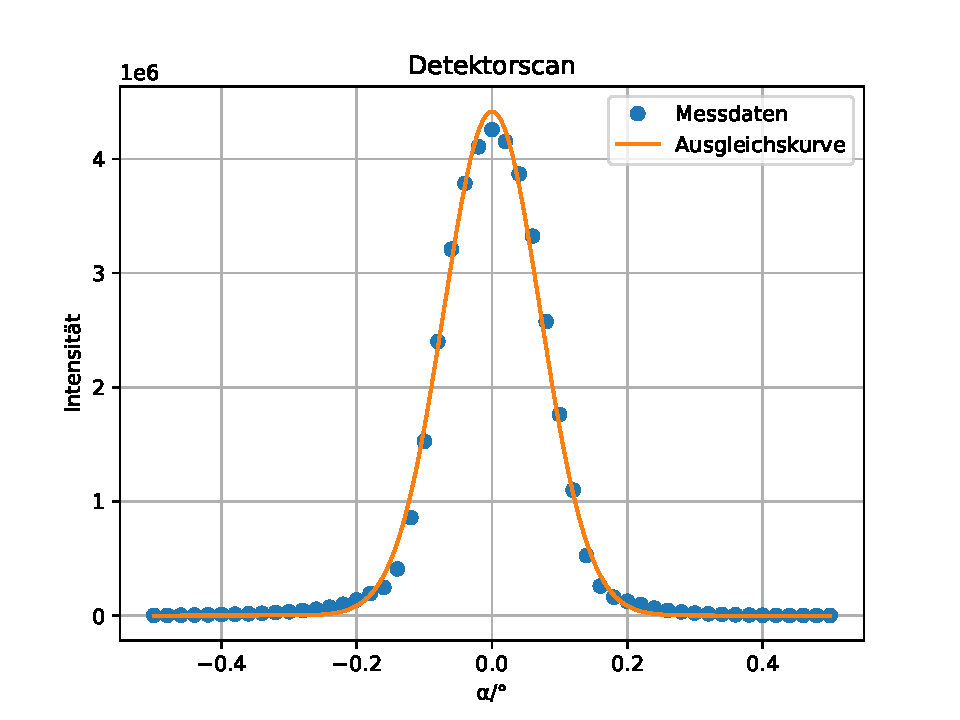
\includegraphics[width = 0.7\textwidth]{Auswertung/Graphen/Detektorscan.pdf}
    \caption{Detektorscan}
    \label{fig:gauß}
\end{figure}
Draus ergibt sich mittels \textit{SciPy} \cite{scipy} eine Amplitude  von $I_{max} =(11,1\pm 0,3) \cdot 10^5$ 
und eine Halbwertsbreite von $(0,246 \pm 0,003)^°$.



\subsection{Z-Scan}
Der Z-Scan ist in Abbildung \ref{fig:Z} dargestellt.
\begin{figure}[h]
    \centering
    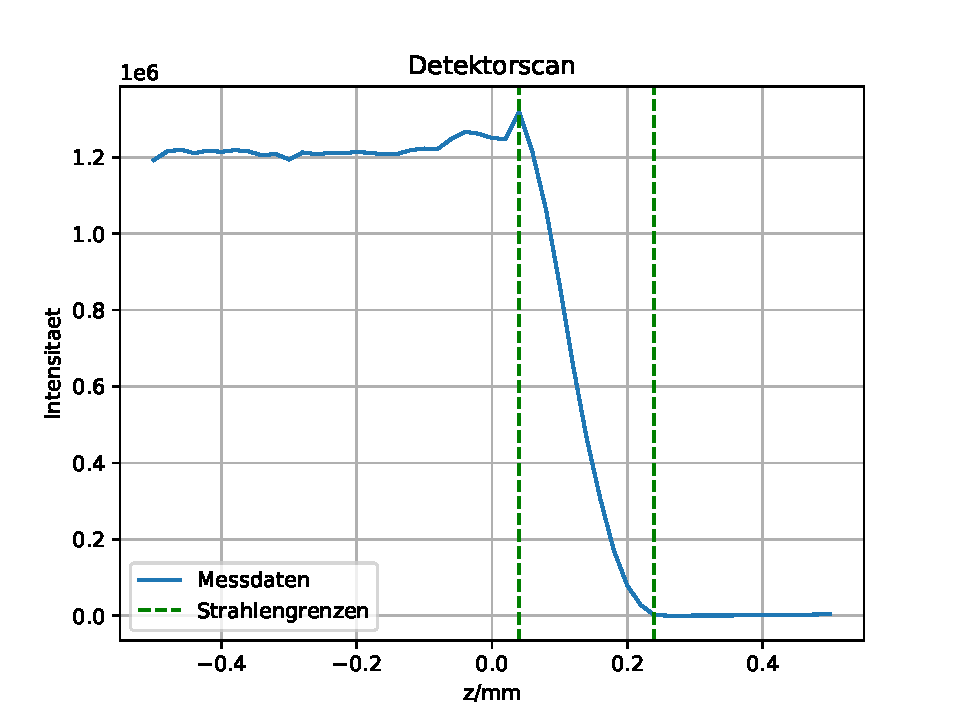
\includegraphics[width = 0.7\textwidth]{Auswertung/Graphen/z_Scan.pdf}
    \caption{Z-Scan}
    \label{fig:Z}
\end{figure}
Zu erkennen ist die Abfallende Intesität, wenn die Probe in den Strahl gefahren wird.
Dies dient neben dem Justieren der Z-Achse ebenfalsss zur Bestimmung der Strahlenbreite $d_0$.
Dies lässt sich als die Differenz zwischen Intensitätsmaximum und Intensitätsminimum ablesen.
Wie in der Abbildung zu erkennnen ergibt diese sich zu $d_0 \approx 1,9$ mm.



\subsection{Rockingscan}
Der durchgeführte Rockingscan ist in Abbildung \ref{fig:roc} dargestellt.
\begin{figure}[h]
    \centering
    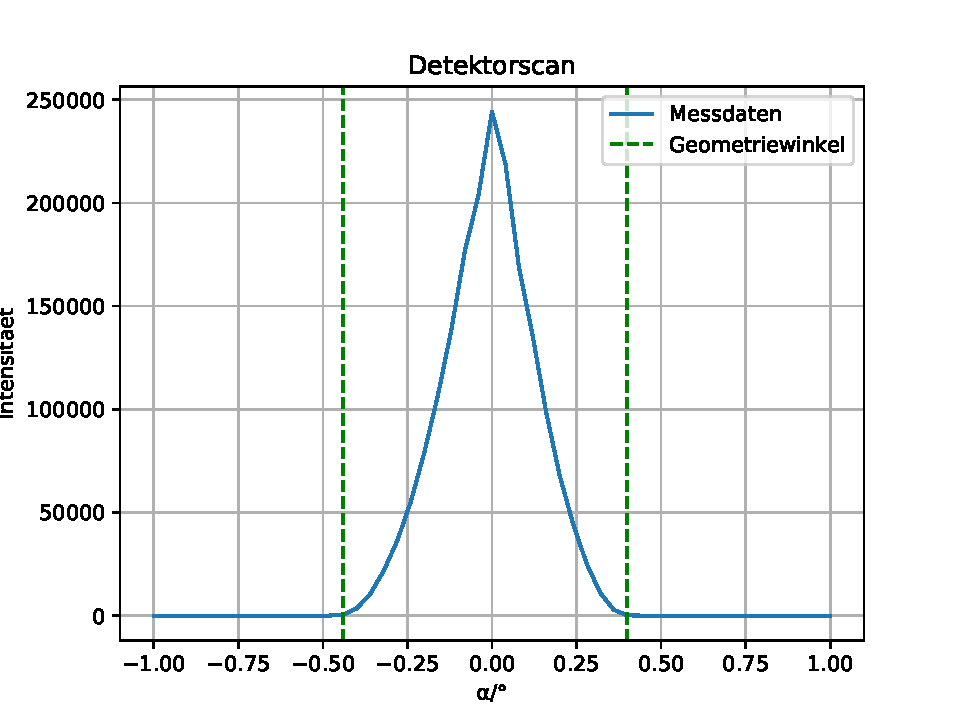
\includegraphics[width = 0.7\textwidth]{Auswertung/Graphen/Rocking_Scan.pdf}
    \caption{Rockingscan}
    \label{fig:roc}
\end{figure}

Daraus lässt sich wie dargestellt der Geomitriewinkel $\alpha_g = 0.4$ ablesen.



\subsection{Reflektivitätsscan}
Die Hauptuntersuchung der Probe findet per Reflektivitätsscan statt.
Um Effekte durch Rückstreuung zu verhindern wird der difuffe Scan vom Reflektivitätsscan subtrahiert.
Dies in Abbildung \ref{fig:ref} dargestellt.
\begin{figure}[h]
    \centering
    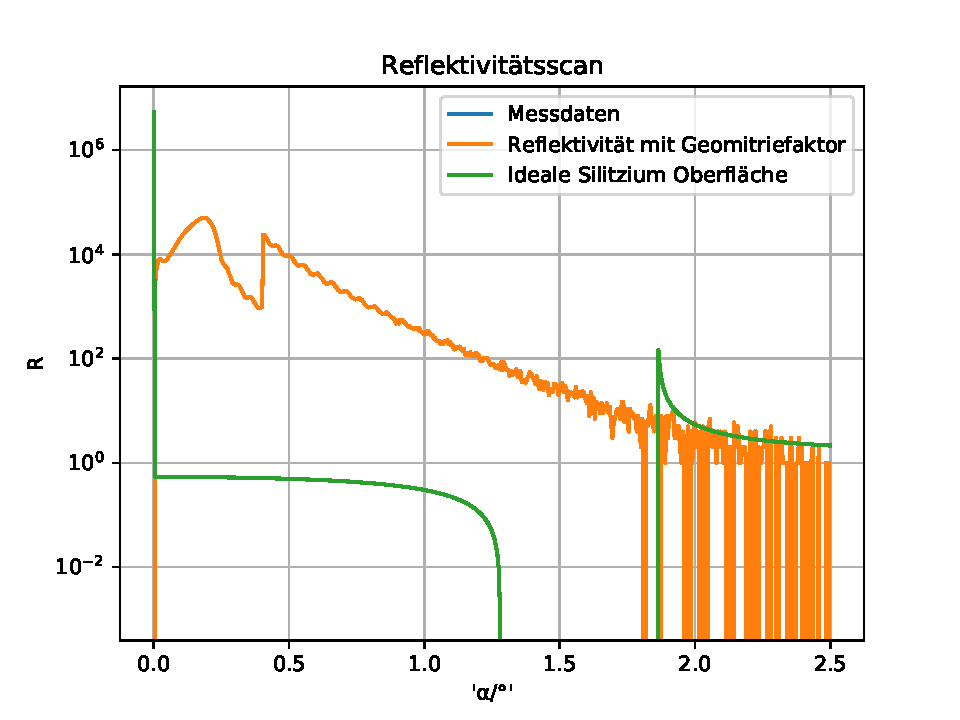
\includegraphics[width = 0.7\textwidth]{Auswertung/Graphen/Reflektivitaetsscan.pdf}
    \caption{Reflektivitaetsscan}
    \label{fig:ref}
\end{figure}
Dabei ist zu beachten das neben dem Winkel die Reflektivität
\begin{equation*}
    R = \frac{I}{5\cdot I_{max}} 
\end{equation*}
aufgetragen wird.
Neben der Reflektivität ist auch die Korrektur durch den Geometriefaktor aufgetragen,
welcher berücksichtigt,
dass erst ab einem gewissen Winkel der komplette Strahl die Oberfläche trifft.
Ebendso ist die berechnete Reflektivität einer Glatten Silizium Oberfläche dargestellt,
welche mittels
\begin{equation}
    R = \left(\frac{\alpha_c}{2\alpha_i}\right)^4
\end{equation}
berechnet wird. 
Der Literatur Wert für den kritischen Winkel $\alpha_c$ liegt für Silizium bei $\alpha_{Si} = 0,223°$ \cite{wert}

Die Schichtdicke lässt sich mit hilfe der Kiesling-Oszillation aus der gemessenen Reflektivität bestimmen.
Dazu werden die auftretenden Minima untersucht und der gemittelte abstand zwischen ihnen bestimmt.
Dabei schaut man sich nur die deutlich auftretenden ersten Minima an.
Der gemittelte Abstand der Minima ergibt sich zu
\begin{equation}
    \Delta\alpha = (4,5 \pm 0,3)\cdot10^{-2}°.
\end{equation}
Mittels der Gleichung
\begin{equation}
    d = \frac{\lambda}{2\Delta\alpha_i}
\end{equation}
ergibt sich daraus eine Schichtdicke von
\begin{equation}
    (1.71 \pm 0,2)\cdot 10^{-8} m.
\end{equation}


\subsection{Parratt-Algorithmus}

Mit hilfe des Parratt-Algorithmus lässt sich das Dispersionsprofil bestimmen,
wie auch die kritischen Winkel von Silizium und Polystrol.
Verwendet werden dazu die modifizierten Frenesselkoeffizienten,
denn dadurch kannm man die Rauhigkeit der Probe mit modilieren.
Das Modell funktioniert mit zwei Schichten, eine aus Polystrol und eine aus Silizium.
Die Umgebungsluft wird als eine Schicht mit der Schichtdicke und der Disperison von $d = \delta = 0$ angenommen.
Die sich so ergebende Kurve ist in Abbildung \ref{fig:parratt} dargestellt.
\begin{figure}[h]
    \centering
    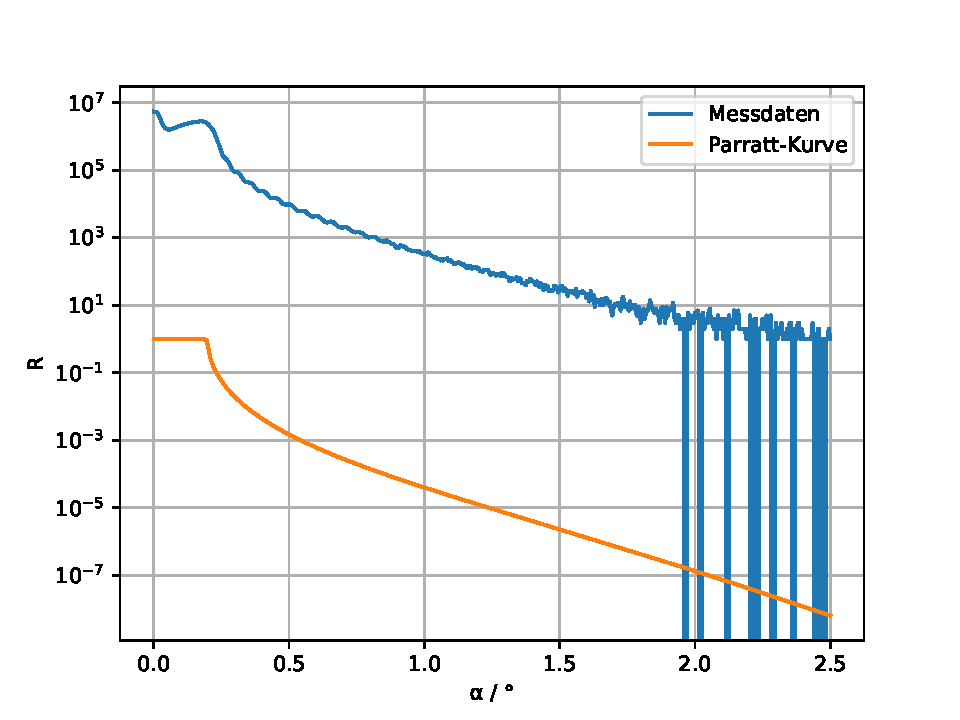
\includegraphics[width = 0.7\textwidth]{Auswertung/Graphen/Parrat_Algorthmus.pdf}
    \caption{Die Parrat Kurve im Vergleich zur gemessenen Reflektivität}
    \label{fig:parratt}
\end{figure}
Mittels der Gleichung \eqref{eq:krit} lässt sich der Kritische Winkel der beiden Schichten jeweils bestimmen als:
\begin{align}
    \alpha_{Pol} &= 0,068^° \\
    \alpha_{Si}  &= 0,214^°
\end{align}
Die Parameter der Schichtdicke $d_2$, der Dispersion $\delta$ und der Rauigkeit $\sigma$ müssen per Hand so bestimmt werden,
dass die Paratkurve eine möglichst große Übereinbstimmung zeigt.
Sie ergeben sich zu
\begin{align*} 
    d_2 &=  1.7\cdot 10^{-6} \\
    \delta_{Poly} &= 7\cdot 10^{-7} \\
    \delta_{Si} &= 7\cdot 10^{-6} \\
    \sigma_{Poly} &=  5.5\cdot 10^{-10}\\
    \sigma_{Poly} &=  6.45\cdot 10^{-10}
\end{align*}
